\documentclass[../../main.tex]{subfiles}

\begin{document}
\problem{54}
\begin{wts}
Did your browser download the two images serially or in parallel? Explain. What are the pros and cons of each approach?
\end{wts}
\begin{proof}
\begin{tikzpicture}
\begin{axis}
[
    title={$V$ against $I$},
    xlabel={$I$ [\text{mA}]},
    ylabel={$V$},
    xmin=0, xmax=16,
    ymin=0, ymax=16,
    xtick={0,4,8,12,16},
    ytick={0,4,8,12,16},
    %legend pos=south west,
    ymajorgrids=true,
    xmajorgrids=true,
    grid style=dashed,
]

\addplot+[
    color=blue,
    only marks,
    mark=square,
    ]
    coordinates {
    (0.8,0.819)(2.1,2.1)(3.2,3.143)(4.1,4.08)(5,5.02)(6.2,6.15)(7.2,7.08)(8.1,8.03)(9,9.04)(10,9.99)(15,14.99)
    };
\end{axis}
\end{tikzpicture}

\noindent\makebox[\linewidth]{\rule{\paperwidth-15em}{0.4pt}}\\[2ex]
A cursory survey of the above plot would suggest that there is a straight line relationship. We now use curve.fit to get our (straight) line of best fit for the data:
%
%
%pgfPlot
%
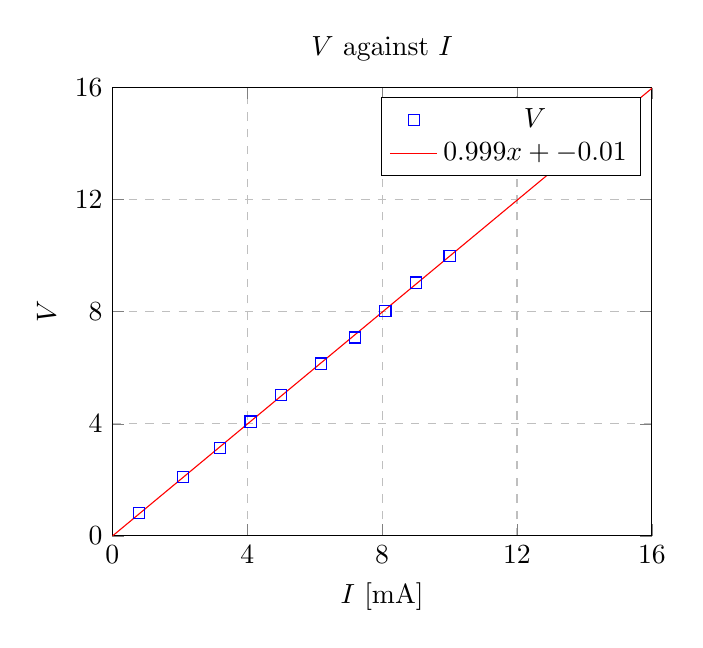
\begin{tikzpicture}
\begin{axis}
[
    title={$V$ against $I$},
    xlabel={$I$ [\text{mA}]},
    ylabel={$V$},
    xmin=0, xmax=16,
    ymin=0, ymax=16,
    xtick={0,4,8,12,16},
    ytick={0,4,8,12,16},
    %legend pos=south west,
    ymajorgrids=true,
    xmajorgrids=true,
    grid style=dashed,
]

\addplot+[
    color=blue,
    only marks,
    mark=square,
    ]
    coordinates {
    (0.8,0.819)(2.1,2.1)(3.2,3.143)(4.1,4.08)(5,5.02)(6.2,6.15)(7.2,7.08)(8.1,8.03)(9,9.04)(10,9.99)(15,14.99)
    };
\addlegendentry{$V$}
\addplot [
    domain=0:20, 
    samples=100, 
    color=red,
]
{0.999*x + -0.01};
\addlegendentry{$0.999x + -0.01$} 
\end{axis}
\end{tikzpicture}


%\caption{\textbf{Curve.fit data: $y=mx+b$\hspace{2mm} Supressing Units.}}
\begin{tabular}{@{}r|l@{}}
\toprule Gradient ($m$) & 0.9986 ± 0.003996\\
y-intercept ($b$) & -0.01245 ± 0.02997\\
Determination Coefficient ($R^2$) & 0.9999\\
\bottomrule
\end{tabular}
\label{tab:fitdata}
\\[2ex]

We conclude, from the high $R^2$ value: Our (straight) line of best fit, fits  well for our given data. Rounding the uncertainty to one significant figure, and rounding the central value to the decimal place of the (rounded) uncertainty:
%\caption{\textbf{Fitted parameters: $y=mx+b$\hspace{2mm} Raw values only, no units.}}
\begin{tabular}{@{}r|l@{}}
\toprule Gradient ($m$) & 0.999 ± 0.004\\
y-intercept ($b$) & -0.01 ± 0.03\\
\bottomrule
\end{tabular}
\label{tab:fitdata}\\[2ex]
\end{proof}

\end{document}